\subsection{Comportamiento electroquímico}

\subsubsection{Cambio de volumen fraccionario}

El cambio de volumen fraccionario calculado con la ecuación \ref{eq:fvc} de la 
sección \ref{ss:electrochim} para las distintas estructuras de Li$_x$Si estudiadas 
se lo presenta en la Figura \ref{fig:fvc}. En la misma se comparan los valores 
obtenidos con datos experimentales de AFM (\textit{atomic force microscopy}) 
medidos por Beaulieu \textit{et al.} \cite{beaulieu2003} y con valores de DFT 
fijos de cambio volumétrico utilizado por Chevrier y Dahn \cite{chevrier2009}. 
Los mismos muestran que el potencial ReaxFF proporciona una tendencia correcta, 
tanto cualitativa como cuantitativamente.
\begin{figure}[h!]
    \centering
    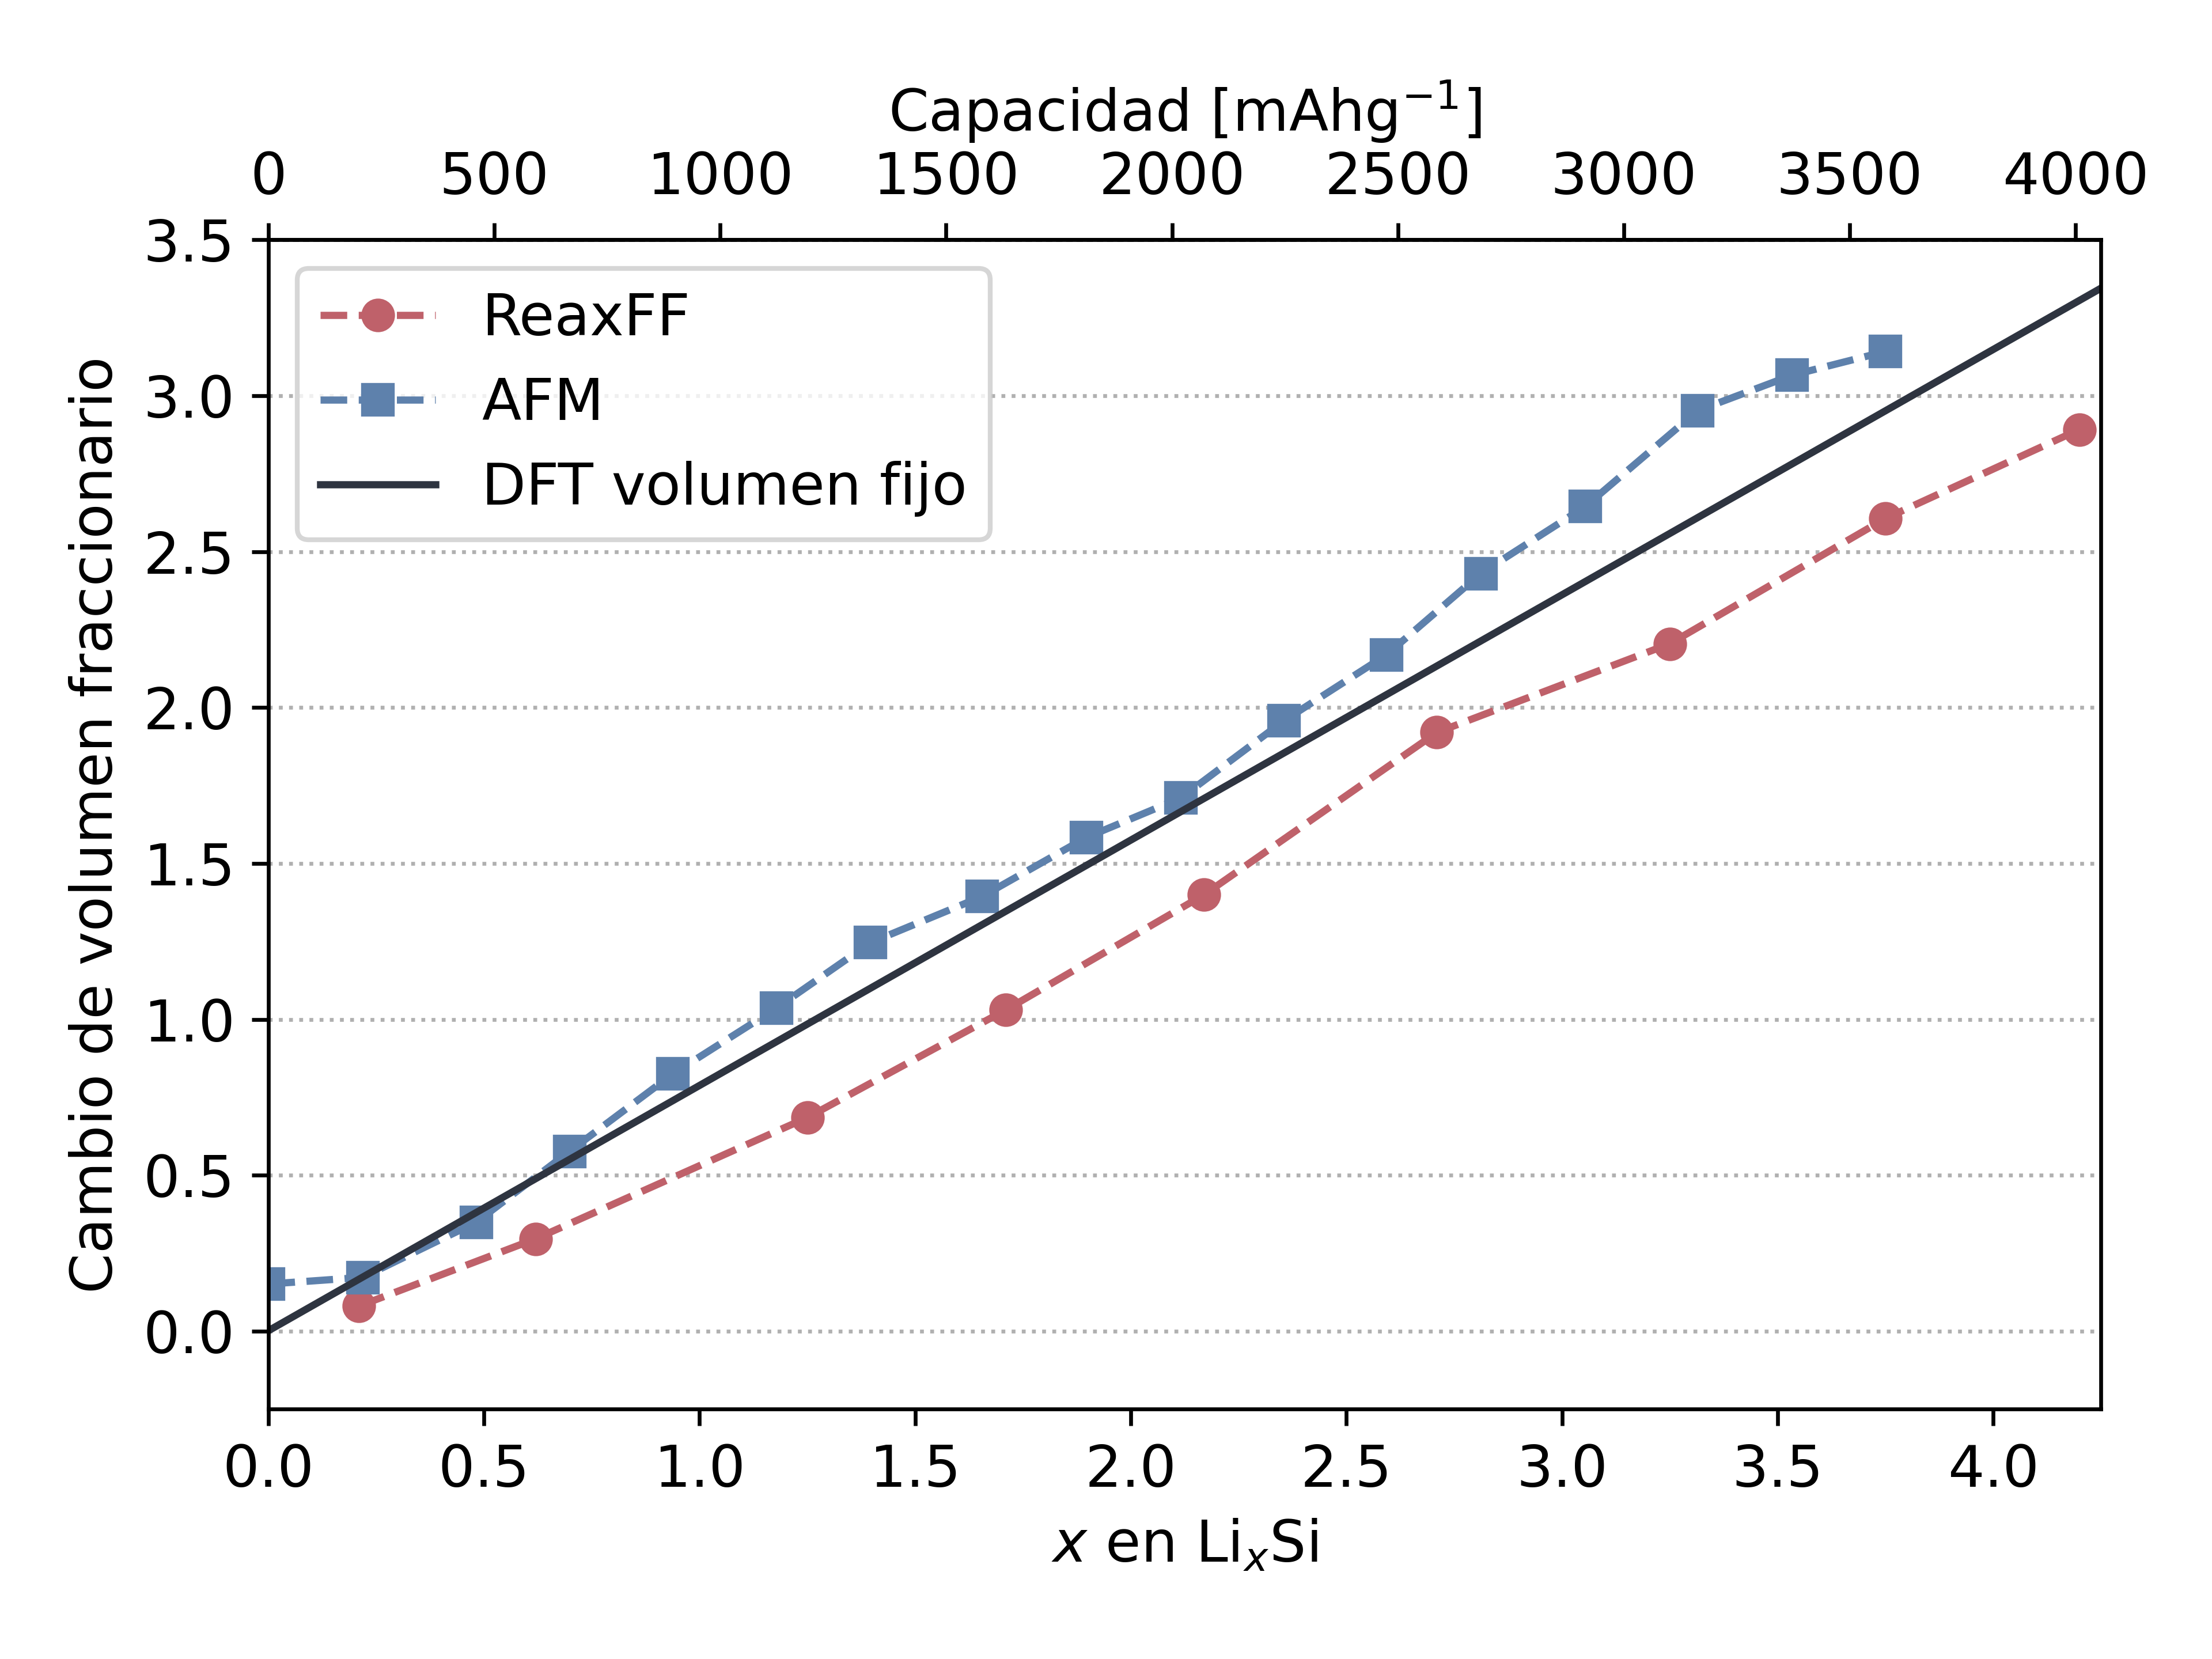
\includegraphics[width=0.8\textwidth]{Silicio/caracterizacion/resultados/electroquimica/fvc.png}
    \caption{Cambio de volumen fraccionario en función de la composición de la 
    aleación. Los valores experimentales de AFM se muestran con cuadrados azules, 
    la línea recta se corresponde con cálculos de DFT y los círculos naranjas son 
    resultados de este trabajo.}
    \label{fig:fvc}
\end{figure}

\subsubsection{Voltaje}

Las energías obtenidas pueden ser utilizadas para evaluar el funcionamiento del 
modelo para predecir propiedades electroquímicas, como fue sugerido por Chevrier
y Dahn \cite{chevrier2009}. Para ello primero se calculan las energías de formación
con la ecuación \ref{eq:formacion} de la sección \ref{ss:electrochim}, que se muestran
en la Tabla \ref{t:fe}. Estas se utilizan luego para calcular el potencial 
\textit{versus} Li metálico de Li$_x$Si, para lo cual se realiza un \textit{spline} 
a estos valores, mostrados en el recuadro de la Figura \ref{fig:voltaje}, se obtienen
los valores de $V(x)$ a partir de la ecuación \ref{eq:voltaje}, que se grafican en 
función de la composición en la Figura \ref{fig:voltaje} con una línea naranja. Para 
comparar, se incluyen en la misma Figura las curvas experimentales medidas para la
litiación y la delitiación de silicio amorfo \cite{hatchard2004} y la curva teórica 
de cálculos de primeros principios \cite{chevrier2009}. Se puede afirmar que los 
resultados obtenidos con el ReaxFF son satisfactorios.
\begin{table}[h!]
    \centering
    \caption{Energías de formación obtenidas a través de la ecuación \ref{eq:fe}}
    \setlength\extrarowheight{2pt}\stackon{%
    \begin{tabular}{c c}
        \toprule
        \textbf{x en Li$_x$Si} & 
        \textbf{Energía de formación [eV]} \\ 
        \midrule
        0.21  &  0.503 $\pm$ 0.003 \\
        0.62  &  0.121 $\pm$ 0.007 \\
        1.25  & -0.12 $\pm$ 0.01 \\
        1.71  & -0.236 $\pm$ 0.007 \\
        2.17  & -0.355 $\pm$ 0.008 \\
        2.71  & -0.410 $\pm$ 0.007 \\
        3.25  & -0.52 $\pm$ 0.01 \\
        3.75  & -0.62 $\pm$ 0.01 \\
        4.20  & -0.699 $\pm$ 0.008 \\
        \bottomrule
    \end{tabular}
    }{}
    \label{t:fe}
\end{table}
\begin{figure}[h!]
    \centering
    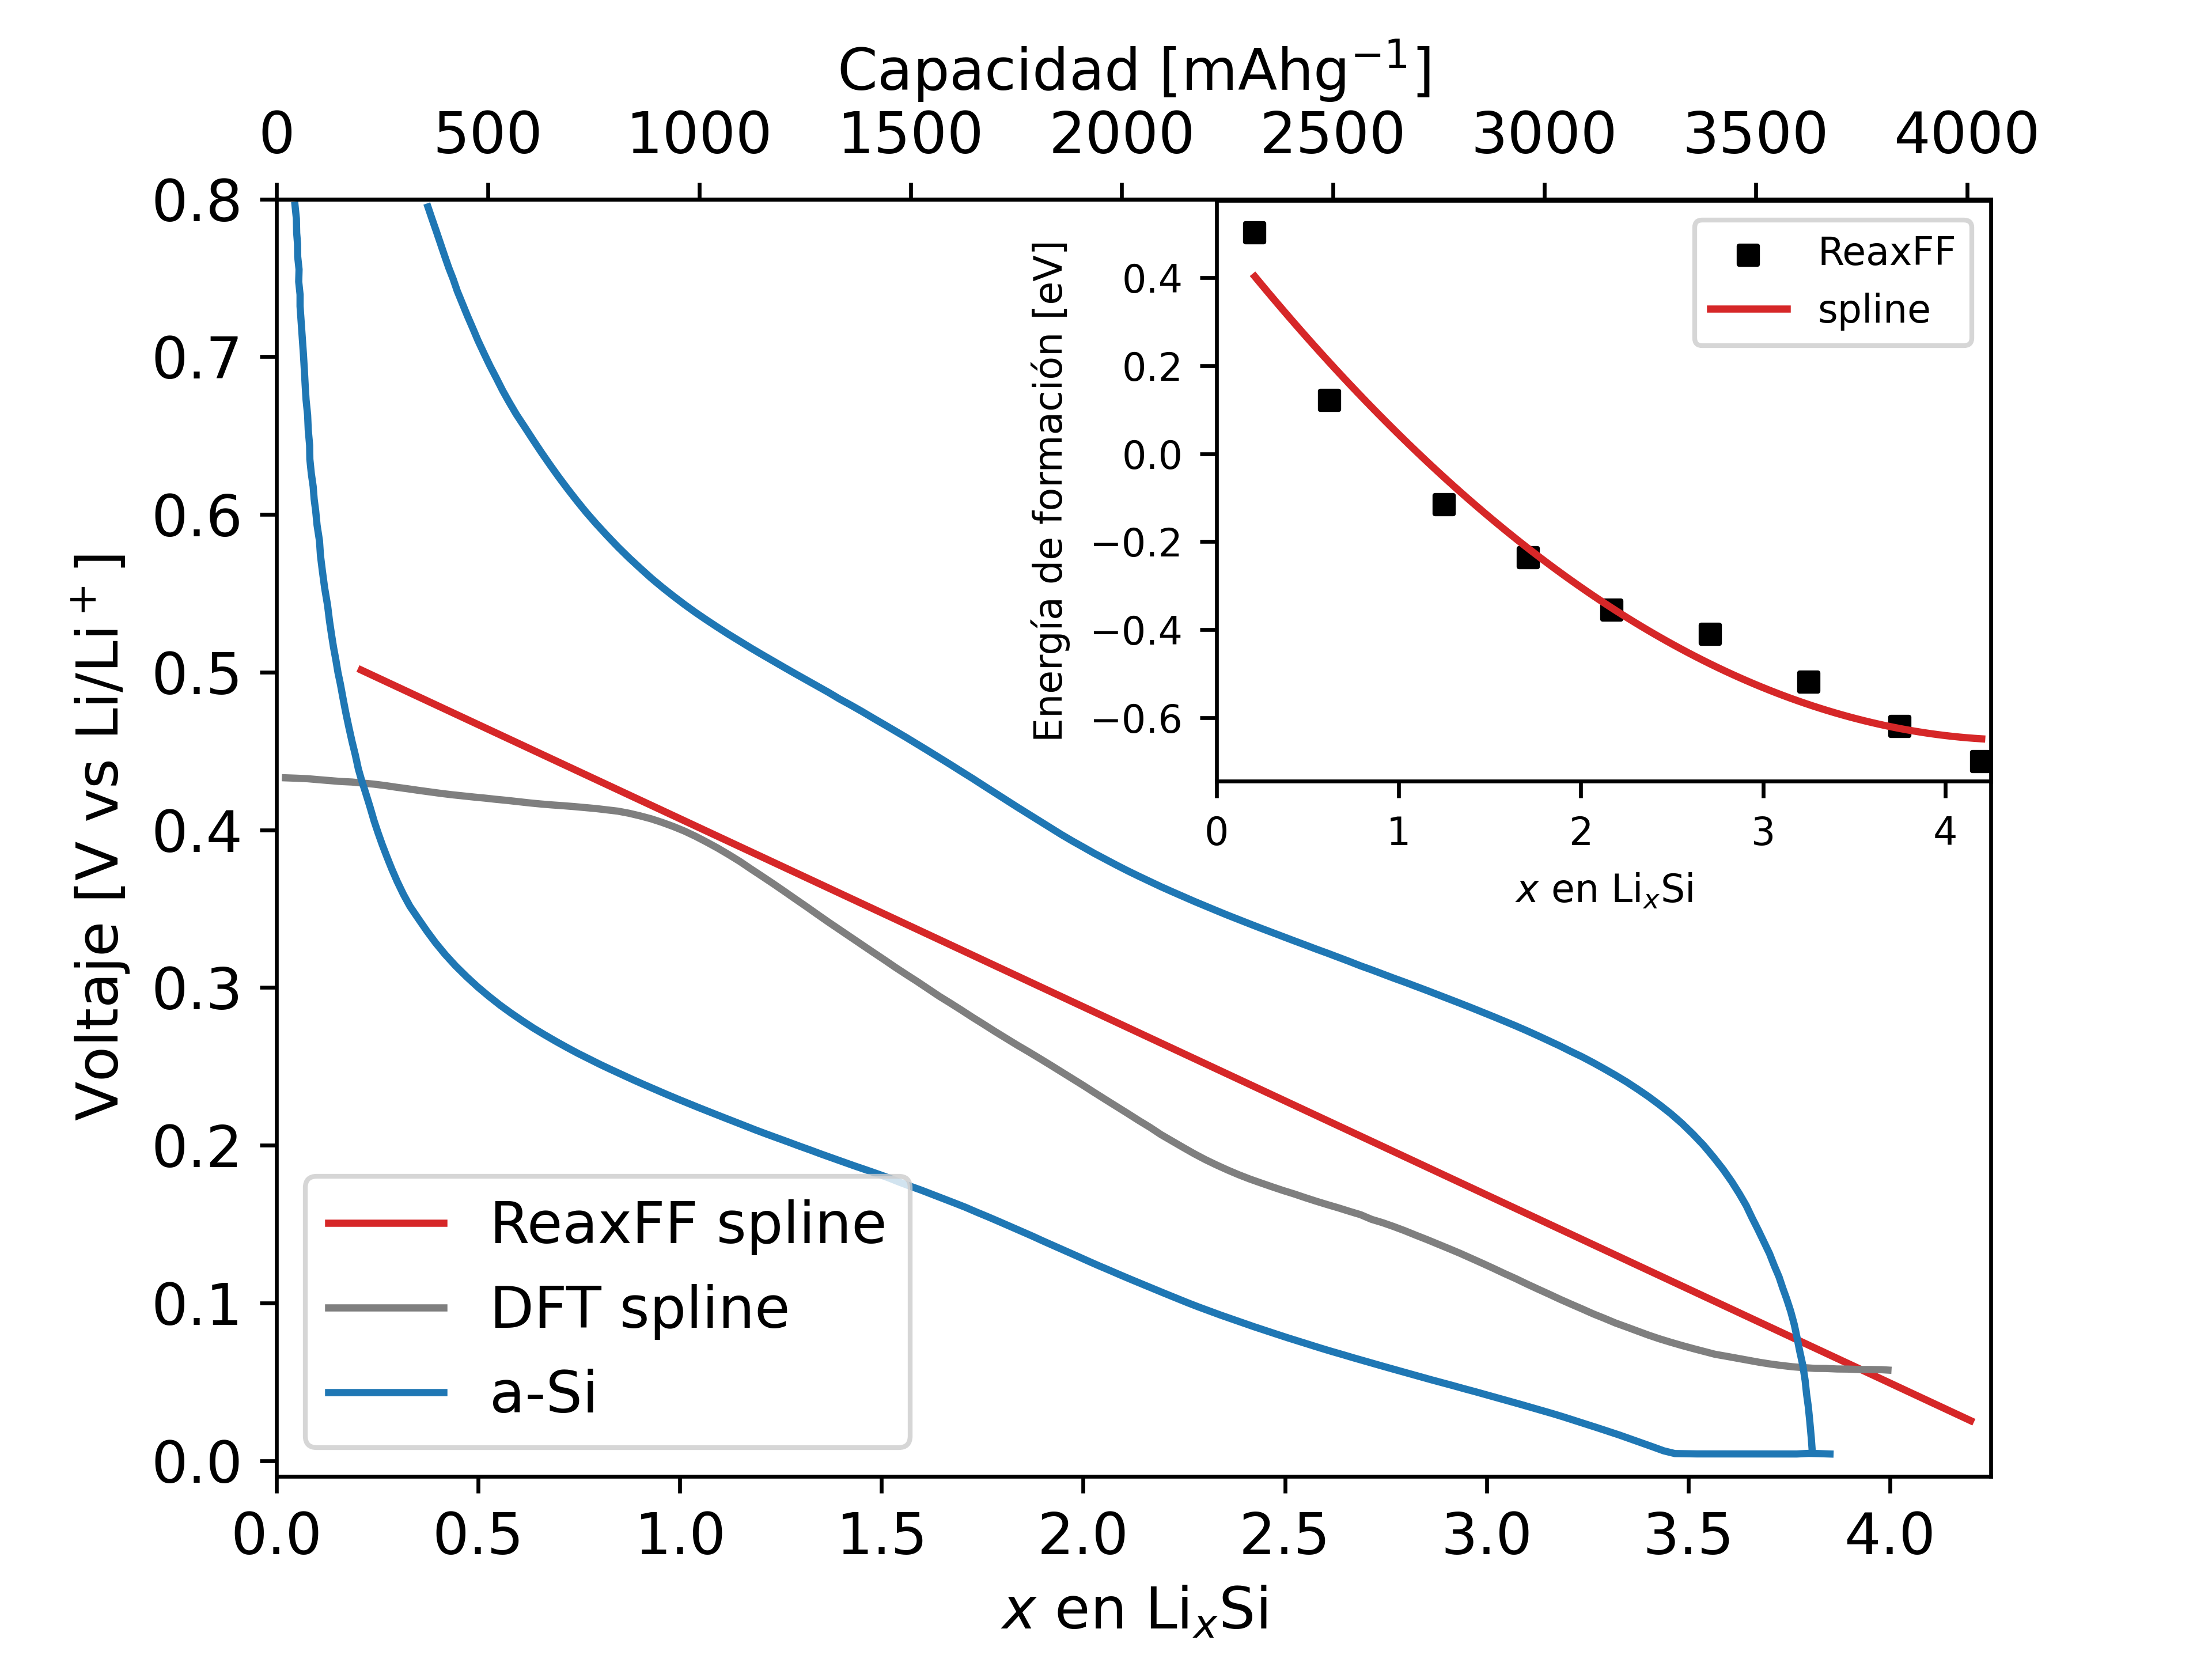
\includegraphics[width=0.8\textwidth]{Silicio/caracterizacion/resultados/electroquimica/voltaje.png}
    \caption{Curvas potencial-concentración para la litiación de ánodos de Si.
    La línea negra corresponde a cálculos de DFT, las líneas azules a 
    curvas medidas experimentalmente en la litiación de Si amorfo y la línea 
    roja es la derivada del \textit{spline} ajustado a los datos de la energía 
    de formación obtenidos con el ReaxFF, presentados en el recuadro.}
    \label{fig:voltaje}
\end{figure}
